\documentclass[a4paper,12pt]{article}

\usepackage{a4wide}
\usepackage{amsfonts}
\usepackage{amsmath}
\usepackage{amssymb}
\usepackage{lipsum}
\usepackage{float}
\usepackage{graphicx}  % For including images

\usepackage{xcolor}  % For a colorfull presentation
\usepackage{listings}  % For presenting code 

\usepackage{hyperref}
\usepackage{xcolor}
\usepackage{listings}

\definecolor{mGreen}{rgb}{0,0.6,0}
\definecolor{mGray}{rgb}{0.5,0.5,0.5}
\definecolor{mPurple}{rgb}{0.58,0,0.82}
\definecolor{backgroundColour}{rgb}{0.95,0.95,0.92}
\lstdefinestyle{CStyle}{
    backgroundcolor=\color{backgroundColour},   
    commentstyle=\color{mGreen},
    keywordstyle=\color{magenta},
    numberstyle=\tiny\color{mGray},
    stringstyle=\color{mPurple},
    basicstyle=\footnotesize,
    breakatwhitespace=false,         
    breaklines=true,                 
    captionpos=b,                    
    keepspaces=true,                 
    numbers=left,                    
    numbersep=5pt,                  
    showspaces=false,                
    showstringspaces=false,
    showtabs=false,                  
    tabsize=2,
    language=C
}
% Definition of a style for code, matter of taste
\lstset{style=CStyle}

%Custom commands
%\renewcommand{\thesection}{Task \arabic{section}}
\newcommand{\ispc}{\textmd{ispc}}

\begin{document}
\title{Assignment 2}
\author{Sophus Valentin Willumsgaard hwx333}
\date{08/12/2024}
\maketitle

% Please leave the table of contents as is, for the ease of navigation for TAs
\tableofcontents % Generates the table of contents
\newpage % Start a new page after the table of contents
%All the programs have been benchmarked on hendrixfut01fl
\section{Programming in \ispc}
For validation and benchmarking, we use the built in test in the c files,
and i will make a note if any of them is modified.
\subsection{Prefix Sum}
I have made the following code. For fun,
I made one version with manual and automatic designation of tasks
respectively to gangs respectively.
\begin{lstlisting}
// First Implementation
export void scan_ispc(uniform float output[], uniform float input[], uniform int n) {
  float currentresult = 0;
  for (uniform int j = 0; j < n; j += programCount) {
    int idx = j + programIndex;
    output[idx] = currentresult + exclusive_scan_add(input[idx]) + input[idx];
    currentresult = broadcast(output[idx],programCount-1);
  }
}
//Second Implementation 
export void scan_ispc2(uniform float output[], uniform float input[], uniform int n) {
  float currentresult = 0;
  foreach (j = 0 ... n) {
    int idx = j;
    output[idx] = currentresult + exclusive_scan_add(input[idx]) + input[idx];
    currentresult = broadcast(output[idx],programCount-1);
  }
}
\end{lstlisting}
This code parses through the validation test.
Running on my personal computer 100 times and taking averages we get
\begin{center}
	\begin{tabular}{ |c|c|c| }
		\hline
		Implementation & Average Runtime \\
		\hline
		C              & 102             \\
		ispc1          & 56              \\
		ispc2          & 56              \\
		\hline
	\end{tabular}
\end{center}
It seems both implementations have the same speed, and that both are faster than the C implementation by a factor
2, which match our expectation.
\subsection{Removing neighbouring duplicates}
We have the following code again with two implementations: First one just
refers to the input directly while the second uses rotate to find the
neighbors
\begin{lstlisting}
//Stupid Implementation: just say you want the previous one from input
export uniform int pack_ispc(uniform int output[], uniform int input[], uniform int n) {
  uniform int m = 0;
  foreach (i = 0 ... n) {
    int j = input[i];
    int cur = input[i-1];
    int keep = j != cur;
    int offset = exclusive_scan_add(keep);
    if (!keep) {
      offset = programCount-1;
    }
    output[m + offset] = j;
    m += reduce_add(keep);
  }
  return m;
}
//(Maybe) Less Stupid Implementation: Use rotate, and manually fix the first index.
export uniform int pack_ispc2(uniform int output[], uniform int input[], uniform int n) {
  uniform int m = 0;
  uniform int last = input[0] + 1;
  foreach (i = 0 ... n) {
    int j = input[i];
    int cur = rotate(j,-1);
    cur = insert(cur,0,last);
    int keep = j != cur;
    int offset = exclusive_scan_add(keep);
    if (!keep) {
      offset = programCount-1;
    }
    output[m + offset] = j;
    last = extract(j,programCount-1);
    m += reduce_add(keep);
  }
  return m;
}
    
\end{lstlisting}
Running the data again 100 times we get
\begin{center}
	\begin{tabular}{ |c|c|c| }
		\hline
		Implementation & Average Runtime \\
		\hline
		C              & 343             \\
		ispc1          & 114             \\
		ispc2          & 134             \\
		\hline
	\end{tabular}
\end{center}
It seems the stupid(?) implementation is slightly faster, but both are
faster than the c code by a factor 3.
\subsection{Run-length encoding}
We have the following code
\begin{lstlisting}
export uniform int rle_ispc(uniform int output[], uniform int input[], uniform int n) {
  uniform int cur = input[0];
  uniform int count = 0;
  uniform int j = 0;
  foreach (i = 0 ... n) {
    int f = input[i];
    if (!all(f == cur)) {
      if (programIndex == 0) {
          for (int k = 0; k < programCount; k++) {
            int next = input[i+k];
            if (next != cur) {
              output[j++] = count;
              output[j++] = cur;
              cur = extract(next,0);
              count = 1;
            } else {
              count++;
        }}
    }} else {
    count += programCount;
    }
  }
  output[j++] = count;
  output[j++] = cur;
  return j;
}
\end{lstlisting}
Since our code is only parallel when every input in a gang is the same, the
code should be very effective for data with a lot of repetition, and less so
for data with less repetition. To test this let us run the code with the
count variable in rle.c first being between 0 and 10, then 0 and 100 and
lastly 0 and 1000
This gives us the results

\begin{center}
	\begin{tabular}{ |c|c|c| }
		\hline
		Implementation & Average Runtime & Max Count \\
		\hline
		C              & 112             & 10        \\
		ispc           & 268             & 10        \\
		\hline
		C              & 57              & 100       \\
		ispc           & 48              & 100       \\
		\hline
		C              & 50              & 1000      \\
		ispc           & 27              & 1000      \\
		\hline
	\end{tabular}
\end{center}
This matches up with our expectation as the higher the count, the more
effective ispc got.
\section{Tree Operations}
all the code for this can be find in trees.fut. Validation code can be found
in validation.fut, and benchmarks in Ex1.fut, Ex2.fut and Ex3.fut. All
benchmarks were run on hendrixfut01fl
\subsection{Implement depths}
for this i have the following code.
\begin{lstlisting}
-- ## Task 2.1
-- These three functions matches steps and does something based on that
local def depthchange (x: step) :i64 =
  match x
  case #u -> -1
  case #d i32 -> 1

local def boolchange (x: (i64,step)) :bool =
  match x
  case (i64,#u) -> false
  case (i64,#d i32) -> true
local def change3 (x: (i64,step)) :(i64,i32) =
  match x
  case (i64,#d i32) -> (i64,i32)
  case (i64,#u) -> (i64,0)

def depths (steps: []step) : [](i64,i32) =
  let depthchange = map depthchange steps in
  let alldepths = map2 (-) (scan (+) 0 depthchange) depthchange in
  map change3 (filter boolchange (zip alldepths steps))
\end{lstlisting}
This code just uses simple maps and map2s, so the expected work is \(O(n)\)
and span is \(O(\log n)\). We then have the following benchmark. Note the
data only contains steps on the form \(\#\text{d i}32\) but that should not
change the performance.
\begin{figure}[H]
	\centering
	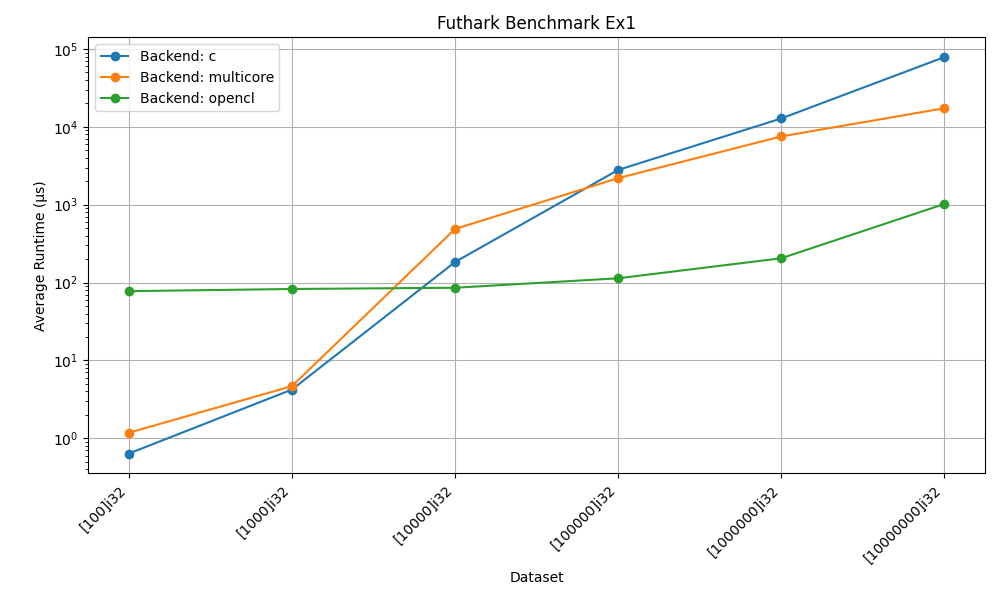
\includegraphics[width=\linewidth]{Ex1benchmark_results.png}
\end{figure}
The data matches our expectation as the c implementation seems mostly to
scale linear, and the opencl implementation remains constant for the first
many cases, suggesting that the span is constant. Since every input has to
be read an implementation would be atleast \(O(n)\) for work, and so it is
efficient.
\subsection{parents}
for this i have the following code\footnote{I didnt have time to figure out
	how to do code hightlighting properly in latex, will try for next one.}
\begin{figure}[H]
	\centering
	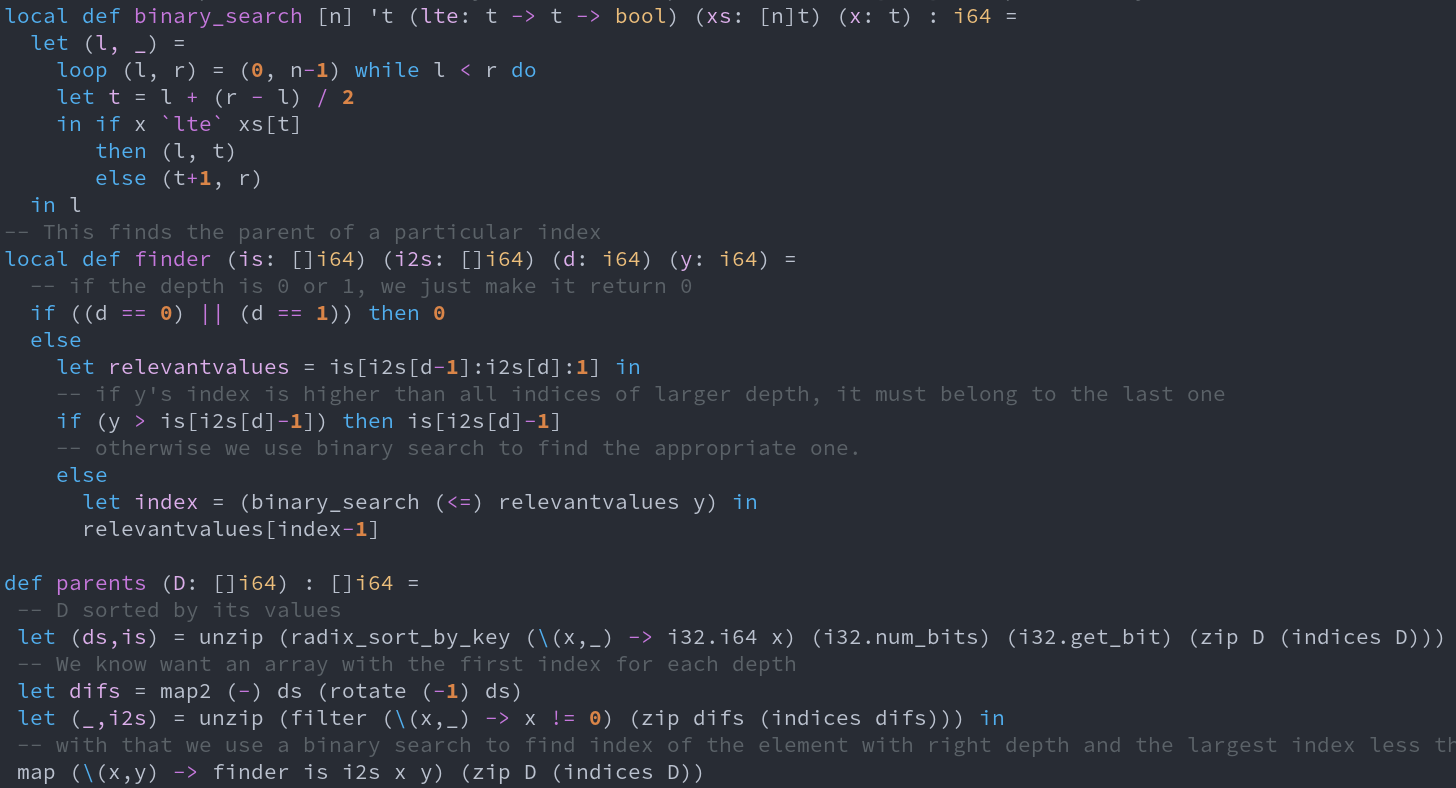
\includegraphics[width=\linewidth]{Ex2.png}
	\caption{}
	\label{fig:}
\end{figure}
Here we have a radix sort, and a binary sort for each element. This should
be done in Work \(O(n \log n)\) time. Meanwhile radix sort is \(S(\log n)\)
and binary sort is \(W(\log n)\)
so we get our span should be \(\log n\).
\begin{figure}[H]
	\centering
	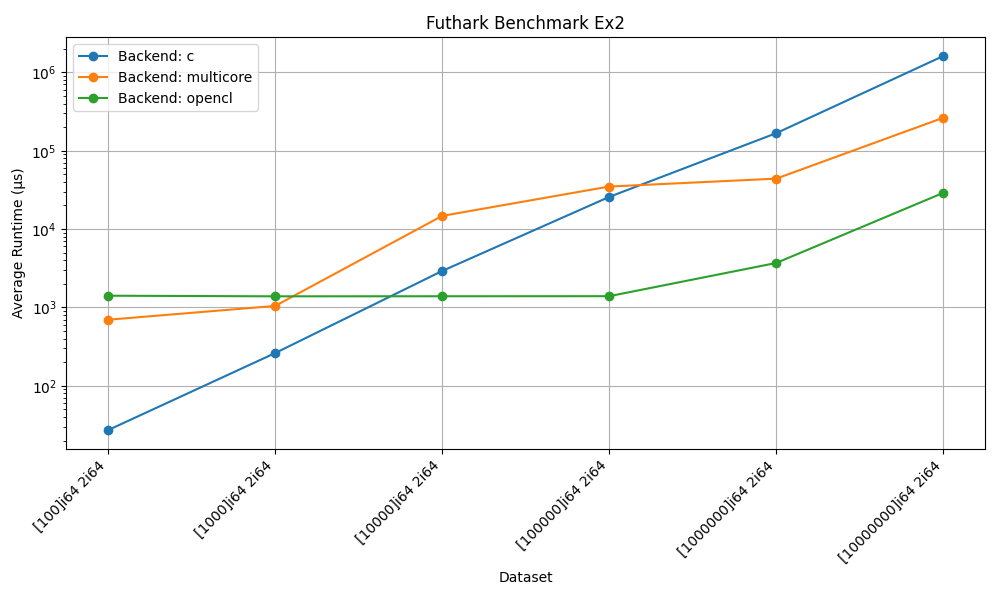
\includegraphics[width=\linewidth]{Ex2benchmark_results.png}
\end{figure}
We see our data matches this. the c implementation is linear while the
opencl remains close to constant. Note in this benchmark data the depth is
very low.
\subsection{Implement subtree sizes}
We have the following implementation
\begin{figure}[H]
	\centering
	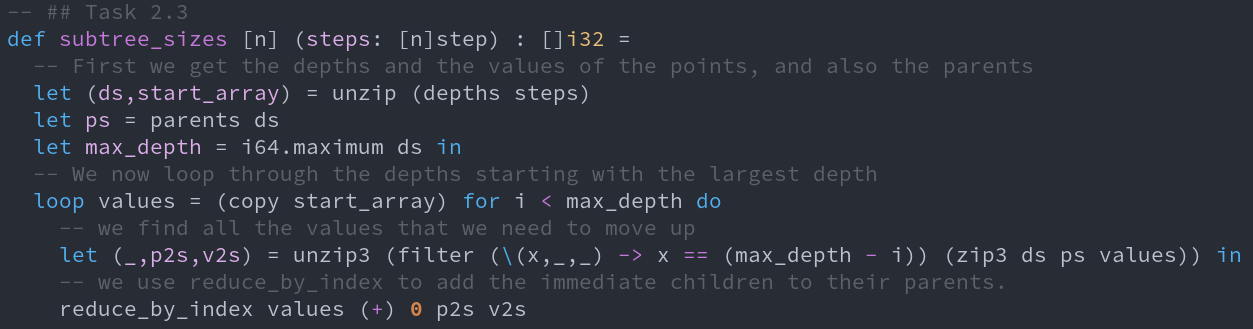
\includegraphics[width=\linewidth]{Ex3.png}
\end{figure}
Here we run depths, and parents, and a reduce\_by\_index max\_depths times.
Since reduce\_by\_index have work \(O(n)\) and span \(O(1)\) (in most
cases), we should expect work \(O(n)\) and span \(O(1)\) for low depths, and
span \(O(n)\) when the tree is close to a line (high depth).
Here we have a low depth benchmark
\begin{figure}[H]
	\centering
	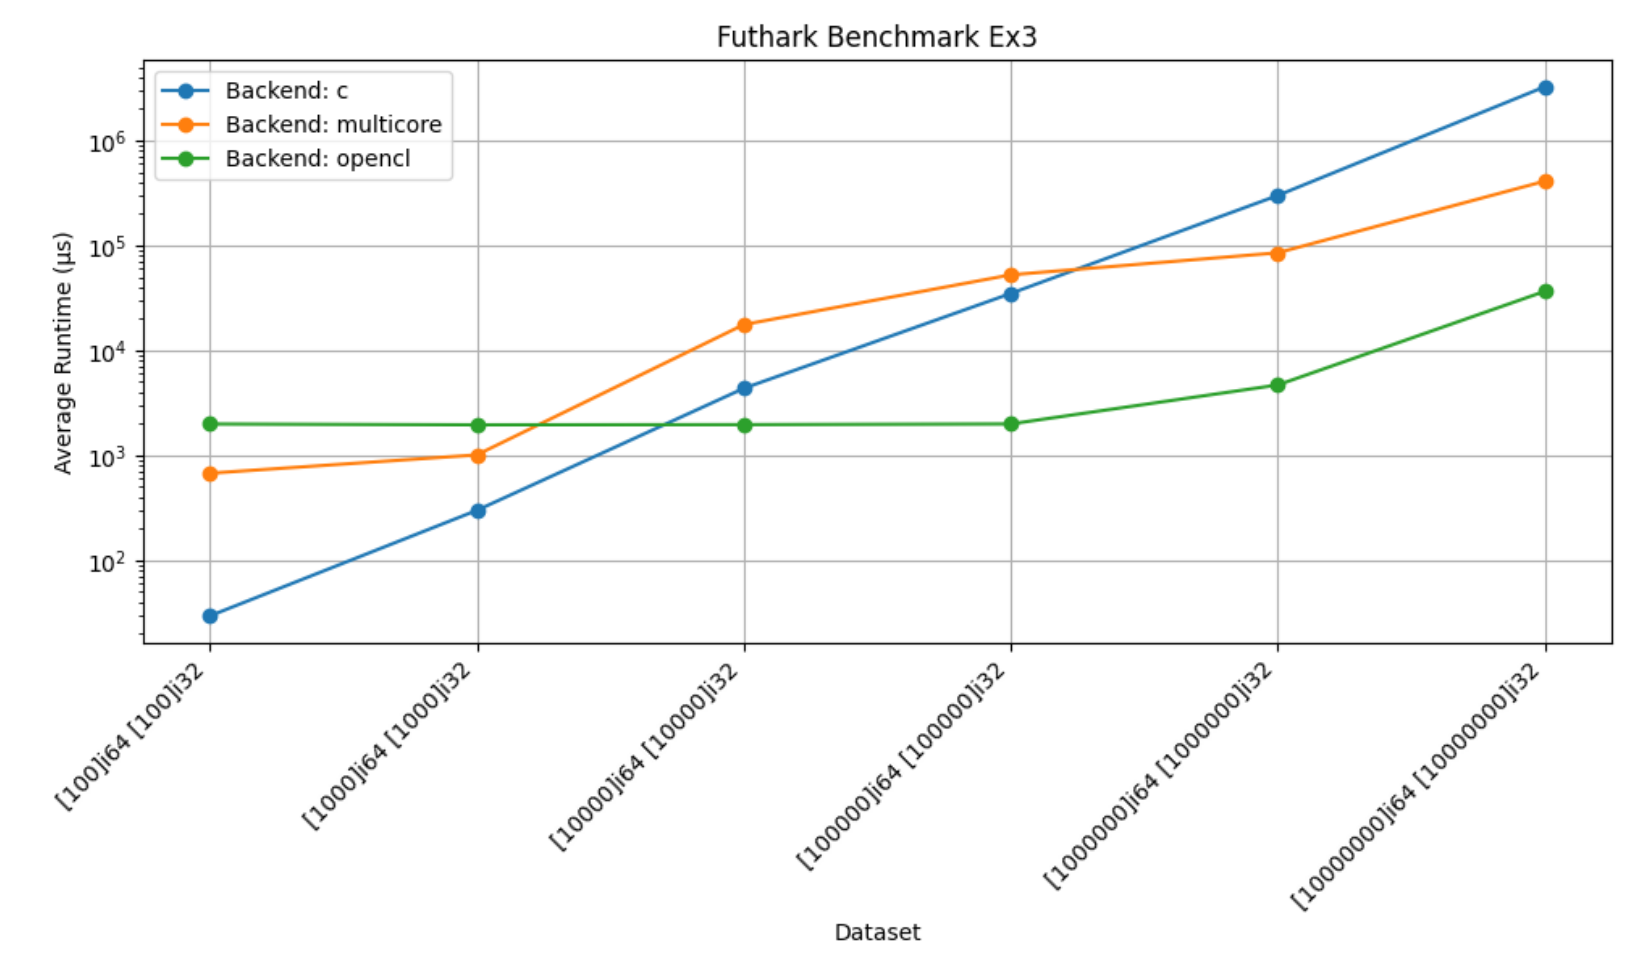
\includegraphics[width=\linewidth]{lowdepth.png}
\end{figure}
again the data matches our expectation. In this graph the tree size is
fixed, but max depth is increased by a factor 10
\begin{figure}[htb!]
	\centering
	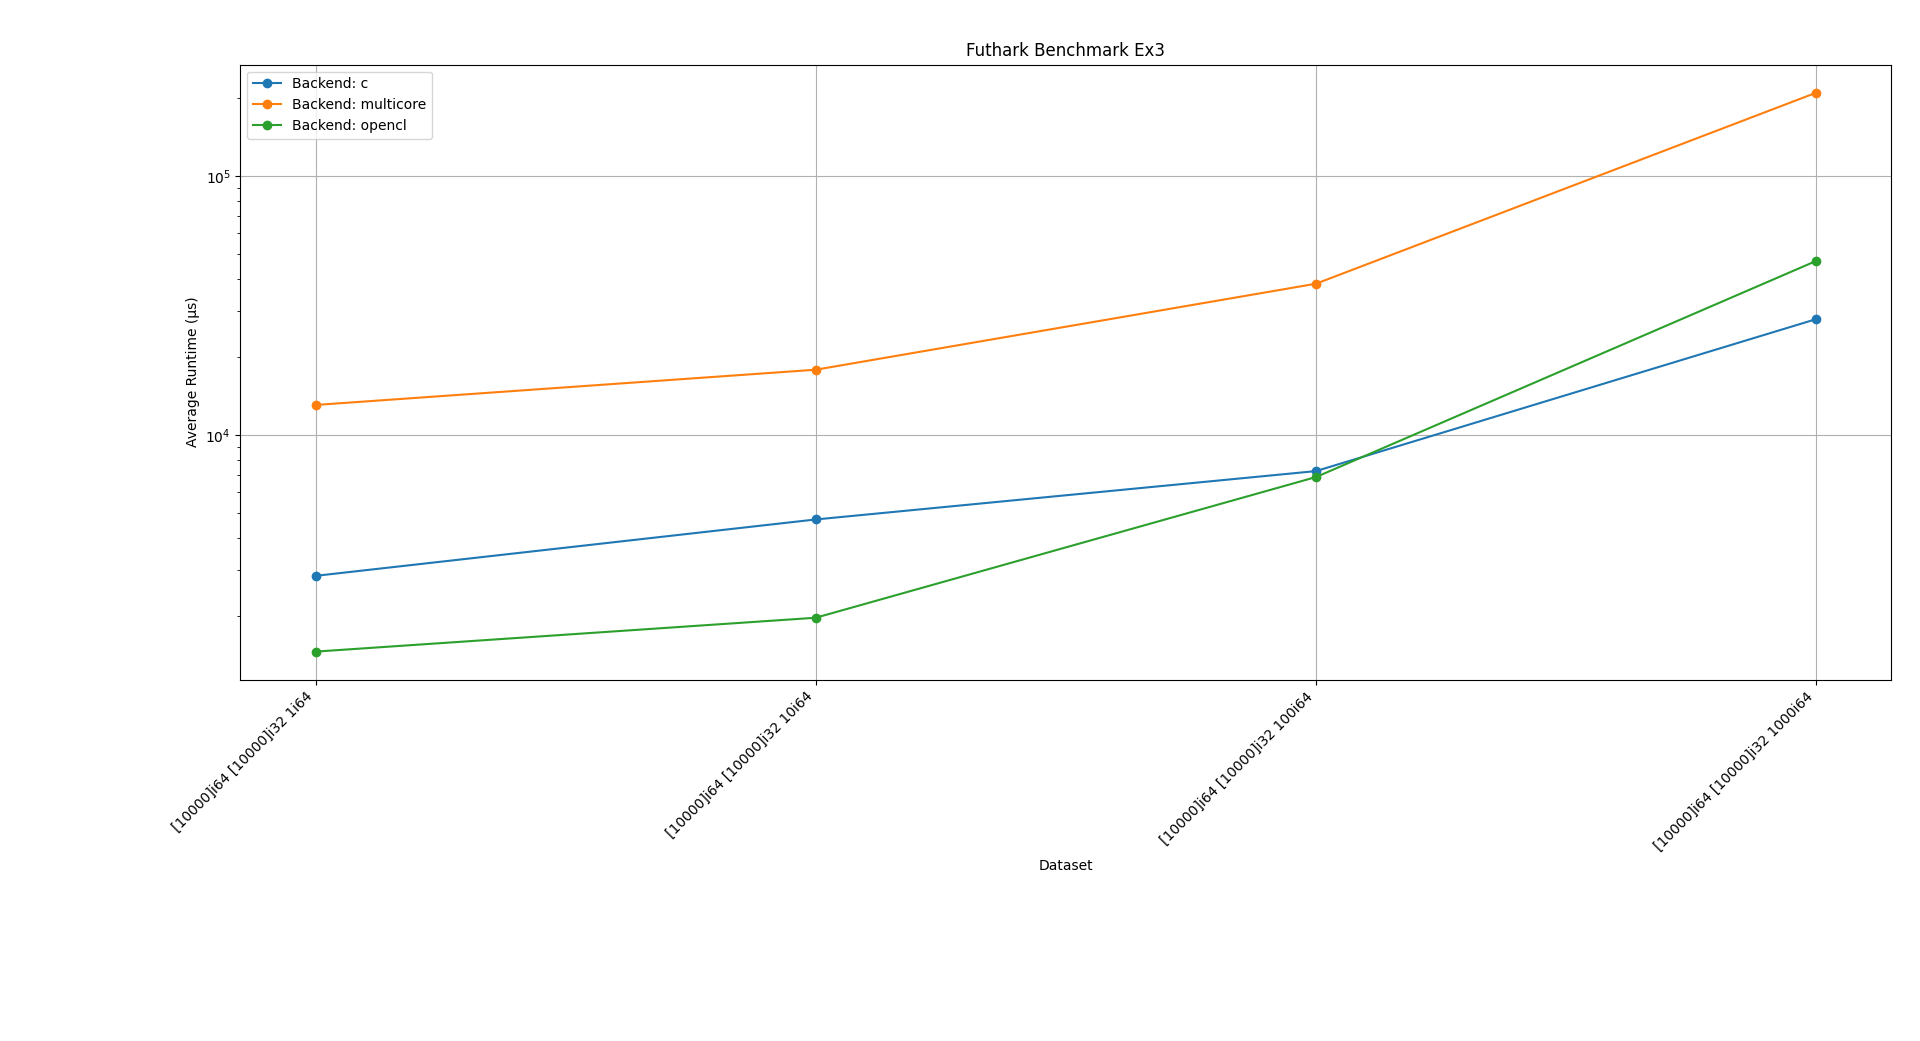
\includegraphics[width=\linewidth]{highdepth.png}
	\caption{}
\end{figure}
We see then that there is no parallel benefit.
\end{document}
